%!TEX root = ../report.tex
\chapter{Background Theory}
%OR: \chapter{Tools and Methods}
\label{cha:background_theory}
\section{Graph theory}
Graph theory is the study of graphs as mathematical structures that models relationships between objects in a collection. A graph consists of vertices connected by edges, \emph{G(V,E)}. In computer science, graph theory is used in areas such as data mining, image segmentation, networking and more\cite{riaz2011applications}. 

\subsection{Graph traversal}
When traversing a graph, two methods are commonly used, breadth first and depth first. Both traversal methods needs a starting point. If there is no natural starting point or root, any vertex in the graph can be selected. Breadth first traversal use a queue containing vertices in the order they are discovered. From the start vertex, all connected vertices are added do the queue, then the first vertex in the queue is visited, and explored. Vertexes connected to the current node is added to the back of the queue, so that the oldest discovered node is the next to be visited. In contrast a depth first search will add newly discovered vertices to the front, so that the newly discovered vertex will be visited next.

Both traversal methods can be used on directed and undirected graphs. On an undirected graph, any vertex discovered can be added to the list of vertices to visit. In a directed graph, only vertices connected by an edge with a direction going from the current vertex, and to another vertex will be followed. Both traversal types can have a termination condition, so that the traversal will stop before traversing the entire graph. 

\begin{algorithm}[H]
    \caption{BFS(Root R)}
    \label{BFS}
    \SetAlgoLined
    \KwResult{BFS}
    Queue $\mathbf{Q}$ ADD(R)\; Tree t \;
    \While{$\mathbf{Q} \neq \emptyset$}{
        e = POP($\mathbf{Q}$) \;
        n = GetNeighbors(e) \;
        $\mathbf{Q}$ ADD(n) \;
    }
\end{algorithm}

\begin{algorithm}[H]
    \caption{BFS(Root R)}
    \label{DFS}
    \SetAlgoLined
    \KwResult{BFS}
    Stack $\mathbf{S}$ ADD(R)\; Tree t \;
    \While{$\mathbf{S} \neq \emptyset$}{
        v = POP($\mathbf{Q}$) \;
        \If{v not discovered}{
            v.setDiscoveered \;
            n = GetNeighbors(v) \;
            $\mathbf{Q}$ ADD(n) \;
        }
    }
\end{algorithm}

\begin{algorithm}[H]
    \caption{MinimumSpanningTreeBFS(Root R, Terms $Q_t$)}
    \label{MinTreeBFS}
    \SetAlgoLined
    \KwResult{Minimum tree containgin terms $Q_t$}
    Queue $\mathbf{Q}$ ADD(R)\; Tree t \; MatchedWords $M_w$ \;
    \While{$\mathbf{Q} \neq \emptyset$}{
        e = POP($\mathbf{Q}$) \;
        \If{e.tokens $\subseteq Q_t$}{
            t ADD(e) \;
            $M_w$.ADD(e.token $\cap Q_t$) \;
        }
        \If{$Q_t$ = $M_t$}{
            Break \;
        }
        n = GetNeighbors(e) \;
        $\mathbf{Q}$ ADD(n) \;
    }
\end{algorithm}


\section{RDF, ontologies, and knowledge graphs}
Knowledge base, ontology and knowledge graph are terms with multiple definitions, and are often used interchangeably. The definitions here are used to clarify what they mean in this paper, and is not a definitive definition.

\subsection{Ontology}
Ontologies contain representations, conceptualization, relations, categorization, and formal naming of data \cite{davies2006semantic}. Ontologies allows for semantic modeling of knowledge. Here knowledge is data that is not ordered in a strict structure. Using ontologies allows data to be better structured, and reason about the semi-structured data.

Structuring an ontology using a framework like RDF creates a knowledge graph. There is no clear definition on exactly what constitutes a knowledge graph. A broad definition of knowledge graph is ``A knowledge graph acquires and integrates information into an ontology and applies a reasoner to derive new knowledge.'' \citep{KGDef} This definition encompasses multiple technologies. Another definition using RDF graphs as a bases is ``We define a Knowledge Graph as an RDF graph. An RDF graph consists of a set of RDF triples where each RDF triple (s, p, o) is an ordered set of the following RDF terms: a subject s $\in$ U $\cup$ B, a predicate p $\in$ U, and an object U $\cup$ B  L. An RDF term is either a URI u $\in$ U, a blank node b $\in$ B, or a literal l $\in$ L'' \citep{KGDefYago}. This latter definition is how knowledge is structured in the data used in this thesis.

\subsection{RDF as knowledge graphs}
Using RDF as a format when modeling knowledge makes it possible to create structured content from semi-structured knowledge. This structure makes knowledge usable for computer, where it previously would have been difficult to extract accurate and exact knowledge. This information can then be presented in a human readable fashion, or it can be used in other fields, like artificial intelligence.

RDF data is organized into triples. Each triple consists of a subject, object, and a predicate. In an RDF triple the subject is a URI or a blank node. The URI when used in the subject identifies an entity, or is an alias gor the vertex in a different language or other variation of an entity. This subject can have relations to objects describing the same entity.

Predicates are always a URI. URIs used for predicates differ from the ones used for subjects and objects in that predicates are of a type. A type is an identifier used to describe the relation between the subject and object.

Objects have the widest range of possible entries. Like subjects and predicates, objects can be URIs. Object URIs can be entity identifiers like subjects, they can be class identifiers, or they can contain some data and a data type. Blank nodes are just that, blank, and literals are an atomic value. 

A fact is a term often used when describing knowledge bases, ontologies and knowledge graphs. Usually a fact is the smallest piece of information in such a system. In a knowledge graph this is a single RFD triple. Another term often used is entity. An entity is a collection of facts, usually from the same article. Entities can be linked together through facts. In such a fact, one entity is used as the subject, the predicate describes the relation, and the object is the other entity. In such a relation both entities will be URIs.

\subsection{Existing knowledge graphs and ontologies}
Currently two of the largest open technologies for knowledge graphs are Yago and DBPedia. Both these projects use automatic extraction from Wikipedia to create the graph, but differ in the ontology used to build the graphs. Yago also includes data from WordNet and GeoNames to accurately assign entities to classes. Both projects use RDF triples to create a knowledge graph.

\subsubsection{Yago}
Yago is an acronym for Yet Another Great Ontology, and is main data source in this paper. The project describes it self as a knowledge base\citep{yago} and an ontology \citep{mahdisoltani:hal-01699874}, but is often described as a knowledge graph by others. In this paper Yago is described as a knowledge graph.

Yago have many entities with facts describing date and spatial data.\citep{yago} Date facts follows the ISO 8601 format, YYYY-MM-DD, and introduces \# as a wildcard symbol. A fact can only hold information on a single point in time, and uses yagoDate as a data type in addition to information on the date.\citep{yago} In a date fact, the object holds the date information, and the predicate describes a connection between subject and date. ``Nidaros\_Cathedral wasCreatedOnDate 1300-\#\#-\#\# .'' In this example the predicate wasCreatedOn is used to describe a relation between the subject and a date.

To describe a time span two facts are required. One of the facts describes a start date, and the second en end date. Since an entity can have multiple date facts connected, all date predicates are also assigned to a class. Start dates are assigned to a predicate with a type that has a ``creation'' class, such as ``StartedOnDate''. End dates are assigned to ``destruction'' type predicates. This makes it possible to deduce a time span for a given subject and predicate combination.\citep{yago}

Yago only contains permanent spatial data for entities on earth. This means that entities like cities, buildings, rivers and mountains are given a spatial dimension. In addition, events, people, groups and artifacts can be given a spatial dimension by relating the entity to a specific place. All spatial facts must have a predicate that fall under the yagoGeoEntity class, and all objects used in a fact with a yagoGeoEntity must have a relation containing both ``hasLatitude'' and ``hasLongitude''.

\begin{figure}[t]
  \centering
  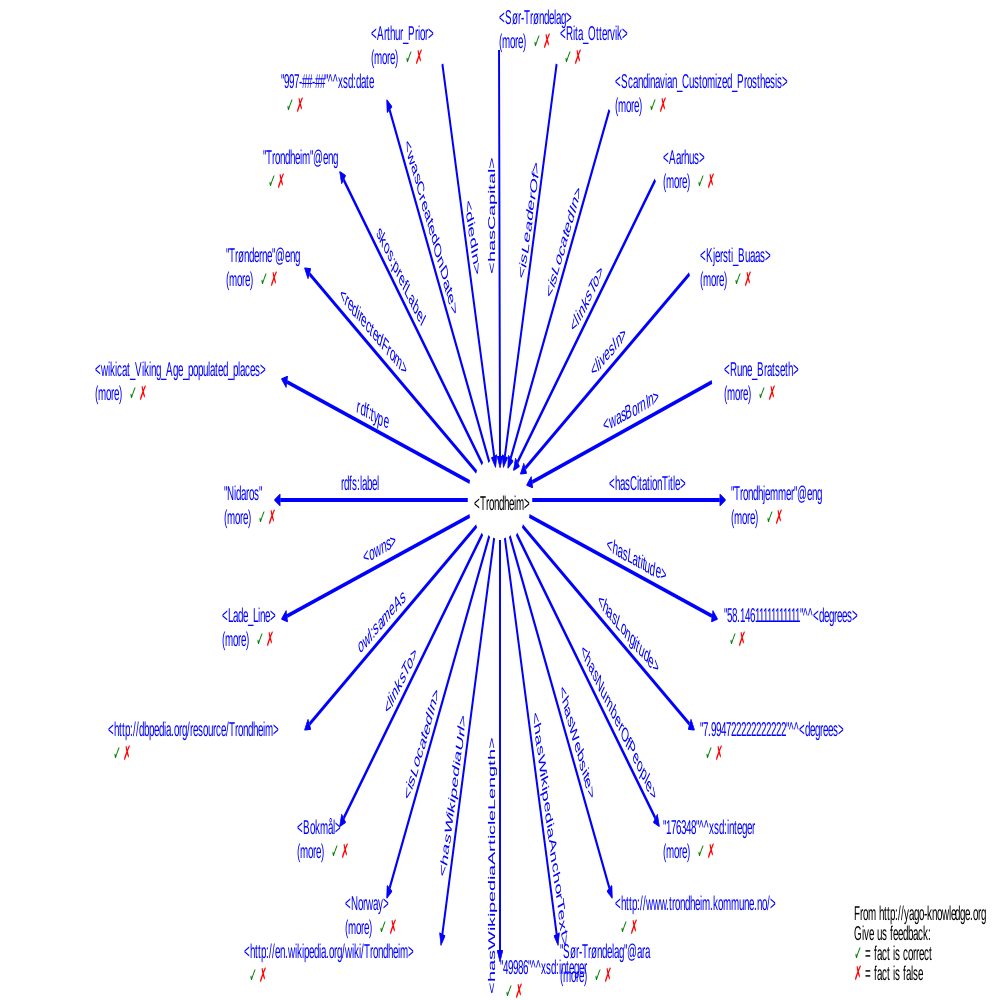
\includegraphics[scale=0.3]{figs/yago_trondheim.png}
 \caption{Trondheim as a subject in YAGO}
 \label{fig:Trondheim}
\end{figure}

\begin{figure}[t]
  \centering
  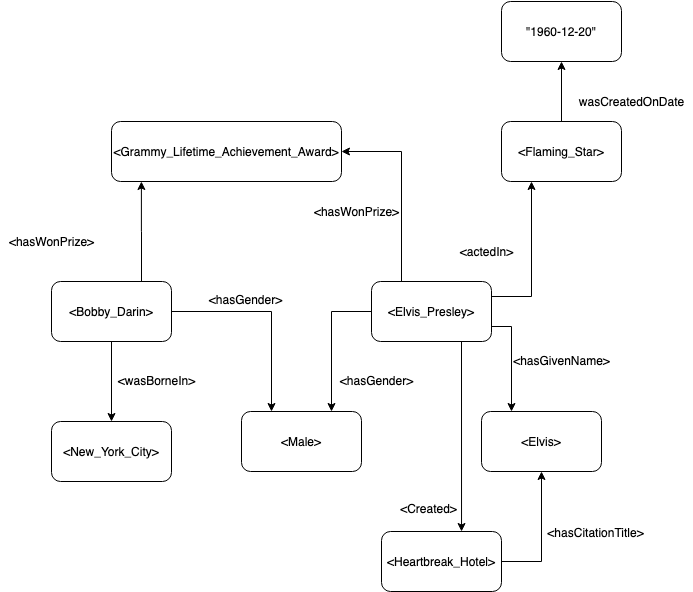
\includegraphics[scale=0.5]{figs/yagoExample.png}
 \caption{Connections in Yago around Elvis}
 \label{fig:Elvis}
\end{figure}

% \subsubsection{DBPedia}

\subsection{Uses for Knowledge graphs}
% One of the more well known uses for ths is inboxes on search engines. These boxes use RDF data to list key facts about the top search result.
One of the uses of knowledge graphs today is to find and display a info box in search engines. This information is a compact set of facts that tries to fit the search query. Because of the graph structure of knowledge graphs the information in the info box can be adapted to the query by choosing the predicates and related facts closest related to the query. This makes it possible to create a set of information that can give the user a quick overview of the information retrieved by the query.

\subsection{Jena}
Apache Jena is a framework for working with semantic web and linked data like RDF. The framework contains tools for SPARQL querying, a query language made specifically for RDF graphs. Jena also contains REST-style SPARQL endpoints making the RDF data easily accessible. Using the existing standards makes it easy to use existing data sets, such as Yago or DBPedia, and build utility on top of that data using some of the tools Jena provides.

Jena provides a persistent storage solution called TDB\footnote{https://jena.apache.org/documentation/tdb/architecture.html}. This storage contains tables for vertices, indexing of triples, and a prefix table. The node table stores the representation of RDF ``terms'', where terms are any vertex, excluding some literals. Excluded literals are the xsd:decimal, xsd:integer, xsd:dateTime, xsd:date, and xsd:boolean types. Each vertex is stored with an ID used when data is loaded, and when querying constant terms. Node to ID mappings are stored as a B+ tree, while the ID to node mappings are stored as a sequential access file. Triples are stored in the triple table as a tuple with three node IDs. The prefix table is used for supporting mappings that are used mainly for serialization of triples. Queries in Jena are run using ARQ, a SPARQL supported query engine.

\glsresetall
